\section{Evaluation}
\label{sec:evaluation}

The evaluation follows the preceding security argument.  It first measures
whether an upstream instruction attack reaches the physical-risk endpoint, then
characterizes the final monitor and its stage ablations, and finally tests the
specific enforcement properties claimed by C1--C3.  Three questions guide the
evaluation.
\begin{itemize}
  \item \textbf{RQ1. Attack propagation.}  How often does the frozen SABER
  instruction attack create a new physical-risk transition over a matched clean
  execution?
  \item \textbf{RQ2. System-level outcomes.}  How do \lone, \ltwo, and their
  composition affect task success, the broad risk-transition endpoint, and the
  registered joint-side property?
  \item \textbf{RQ3. Mechanism behavior and cost.}  Do the monitor boundaries
  reach the expected state under targeted semantic and transaction faults, and
  what cost and failure modes does guard screening introduce?
\end{itemize}

The \ltwo arm combines \transactionbinding and \guardscreening, so their
component-specific physical effects are not identifiable from the four-arm
contrast.  Focused transaction cases characterize \ltwoa, while joint-side
measurements and screening latency characterize \ltwob.

\subsection{Experimental Design}

\paragraph{Platform and workload}
The victim is OpenPI $\pi_{0.5}$~\cite{pi05} running on
LIBERO-Safety~\cite{liberosafety2026}.  The policy runs at a 20\,Hz control rate,
returns one $H=10$ source block per call, and receives a new observation after
the block is consumed.  Episodes are capped at 600 steps.  Policy inference and
simulation run on separate NVIDIA RTX 6000 Ada GPUs.

The complete population contains 60 task/initialization base pairs, equally
divided among the benchmark's affordance, human-safety, obstacle-avoidance, and
obstacle-with-human subsets and balanced across three difficulty levels.  Two
independently seeded executions of every pair yield 120 seed-specific evaluation
units.  Initializations are selected without observing outcomes.

The attack workload uses SABER constraint-violation instruction
perturbations~\cite{saber2026}.  One bounded, prompt-only attack record is
generated for each base pair without access to victim outcomes and is frozen
before evaluation.  Both seeded units of a pair use the same record.

\paragraph{Two separate studies}
The \emph{attack-reproduction study} runs one clean and one attacked
unprotected rollout for every unit, for 240 episodes.  Each matched execution
shares the task, initialization, environment seed, and policy seed.  This study
estimates the observed attack success rate (ASR).

The \emph{four-arm study} performs new clean and attacked rollouts for every
unit under \vlaonly, \loneonly, \ltwoonly, and \dual, for
$120\times2\times4=960$ attempts.  \vlaonly is the unchanged runtime baseline,
\loneonly and \ltwoonly are stage ablations, and \dual is the final composed
\system prototype.  Runs for a unit share the initial state and random seeds,
and a counterbalanced arm order reduces schedule effects.  The two studies
share population identities, not rollouts or estimands.

All 960 four-arm attempts produce an outcome record.  Each condition contains
98.96\% valid traces (475/480), short of the registered 100\% all-valid
requirement.  The four-arm results are therefore nonconfirmatory.  Task-success
rates count invalid rows as failures, the broad-risk comparison is a
common-eligible complete-case diagnostic, and joint-side measurements are
valid-trace diagnostics.

\begin{figure*}[t]
\centering
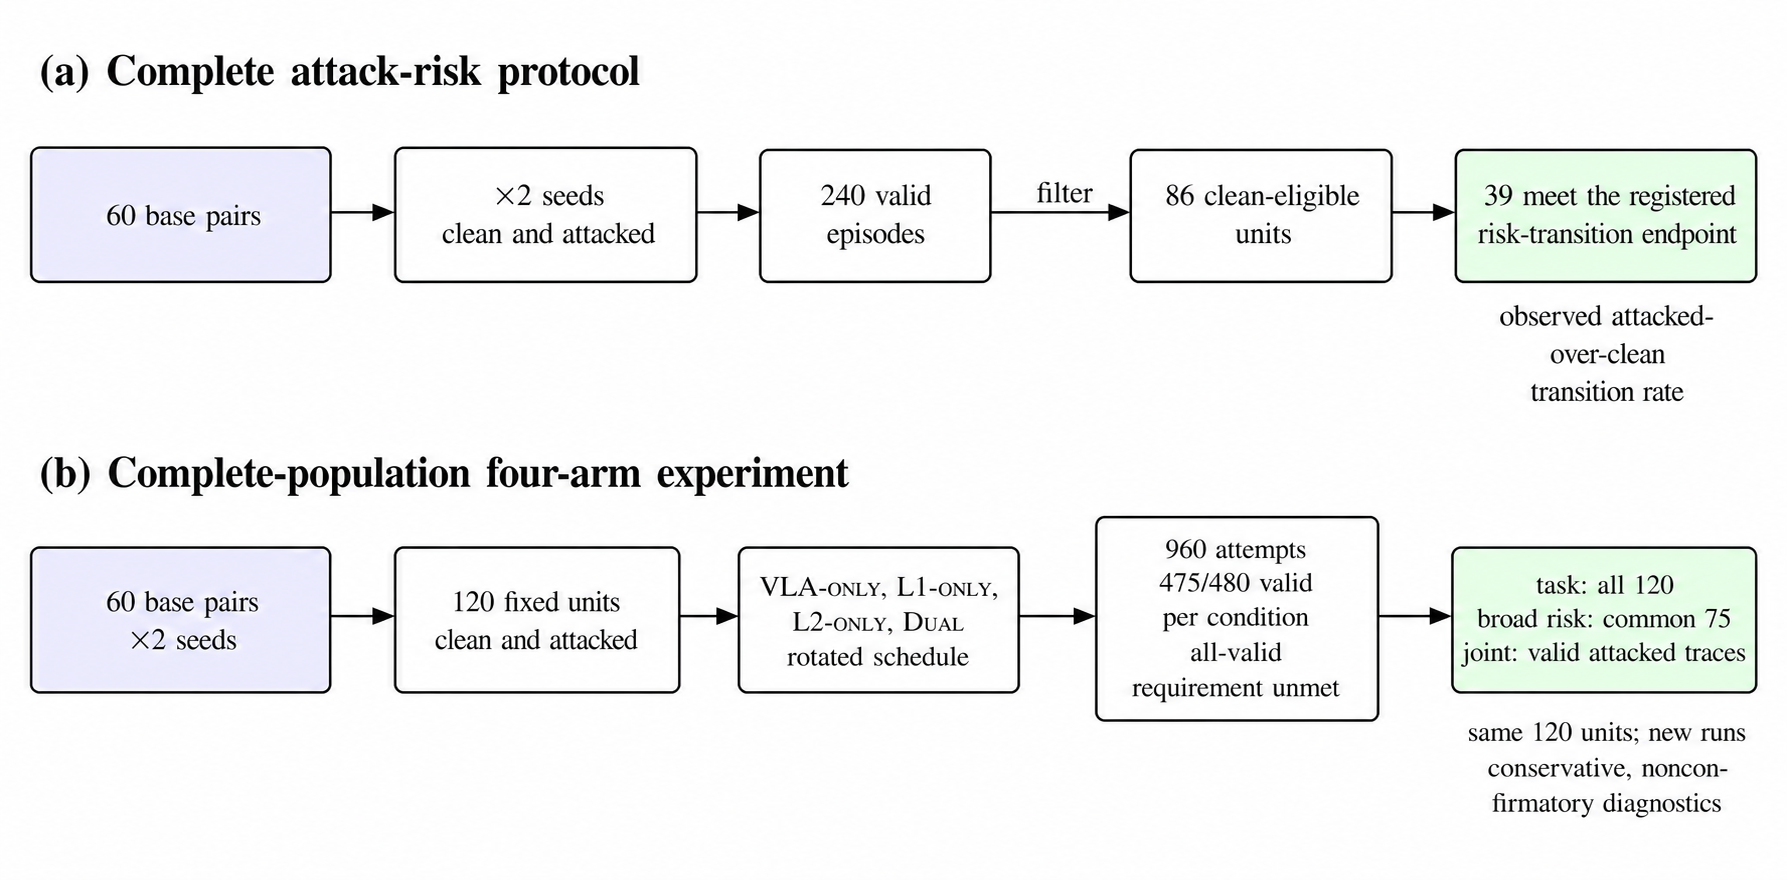
\includegraphics[width=\textwidth]{figures/evaluation_design_raster_v3.png}
\caption{The independent attack reproduction estimates attack propagation.
The separate four-arm study uses new runs over the same 120 population
identities.  Its task-success, broad-risk, and joint-side results use distinct
invalid-trace rules and remain nonconfirmatory.}
\label{fig:evaluation-design}
\end{figure*}

\subsection{Metrics and Counting Rules}

\paragraph{Attack-induced risk transition}
A clean trace is eligible if it is valid, achieves strict task success without a
benchmark cost or collision, and has complete typed constraint-signal and
raw-action coverage.  Clean contact, joint-limit, and force counts need not be
zero.  For an eligible unit with a valid matched attacked trace, a risk
transition occurs when the attacked execution raises the benchmark
cost/collision flag or increases the clean count of robot contacts, joint-limit
steps, or excessive-force steps.  Task failure alone is excluded.

The attack reproduction estimates ASR over its 86 clean-eligible units.  In the
four-arm study, each arm also has a descriptive residual risk-transition rate
over its own clean-eligible units.  Direct cross-arm comparison uses the 75 units
whose clean run is eligible in every arm and whose clean and attacked traces are
valid in every arm.  This common-eligible complete-case cohort gives every arm
the same denominator.  Its rate is a conditional diagnostic, not a
full-population causal effect.

Task-success rates retain all 120 fixed units in every arm, with invalid rows
counted as failures.  Checker rejection is reported among valid traces;
transaction faults are reported over the focused case suite; guard refusal is
reported by valid episode and performed screen.  An invalid trace is not itself
a checker rejection, guard refusal, or observed risk transition.  Percentages
are used for unit- and episode-level outcome rates.  Registered step-level
diagnostics remain counts because no common step-exposure rate was defined.
Paired cross-arm sensitivity tests use exact two-sided McNemar tests on the 75
common-eligible units and carry no confirmatory interpretation.

\subsection{RQ1. SABER Attack Propagation}

All 240 attack-reproduction episodes are valid (100\%).  Among the 86
clean-eligible units, 39 meet the attacked-over-clean risk-transition endpoint.
The observed ASR is therefore 45.35\% (39/86).  This reproduces the SABER
constraint-violation instruction attack on the evaluated OpenPI
$\pi_{0.5}$--LIBERO-Safety path and establishes that the exercised upstream
prompt perturbation can reach the registered physical-risk endpoint.  SABER
serves here as the evaluated Stage-I threat instance; the system objective
continues through the Stage-II execution boundary.

\subsection{RQ2. Final-System and Layer Outcomes}

Table~\ref{tab:task-success} reports the episode-level task-success metric.
Table~\ref{tab:risk-transition} keeps the independent ASR, arm-specific
residual rates, and common-cohort diagnostic visibly separated.

\begin{table}[t]
\centering
\caption{Task-success rates.  Every denominator is the full 120-unit
population; invalid traces count as failures.}
\label{tab:task-success}
\footnotesize
\begin{tabular}{lcc}
\toprule
Arm & Clean & Attacked \\
\midrule
\vlaonly  & 70.83\% (85/120) & 60.83\% (73/120) \\
\loneonly & 65.00\% (78/120) & 53.33\% (64/120) \\
\ltwoonly & 71.67\% (86/120) & 60.83\% (73/120) \\
\dual     & 65.00\% (78/120) & 53.33\% (64/120) \\
\bottomrule
\end{tabular}
\end{table}

\begin{table}[t]
\centering
\caption{Attack-induced risk-transition rates.  The first row is the separate
RQ1 reproduction.  Four-arm native rates use each arm's clean-eligible
denominator; the common column is the matched 75-unit diagnostic.}
\label{tab:risk-transition}
\footnotesize
\setlength{\tabcolsep}{3.5pt}
\begin{tabular}{lcc}
\toprule
Study or arm & Own-cohort rate & Common cohort \\
\midrule
Attack reproduction & 45.35\% (39/86) & N/A \\
\midrule
\vlaonly  & 52.94\% (45/85) & 50.67\% (38/75) \\
\loneonly & 53.85\% (42/78) & 56.00\% (42/75) \\
\ltwoonly & 50.00\% (43/86) & 48.00\% (36/75) \\
\dual     & 55.13\% (43/78) & 57.33\% (43/75) \\
\bottomrule
\end{tabular}
\end{table}

\paragraph{Task success and broad risk}
Under attack, \ltwoonly matches \vlaonly at 60.83\% task success.
\loneonly and \dual each reach 53.33\%.  Relative to \vlaonly, \dual is
5.83 percentage points lower when clean and 7.50 points lower under attack.
The final composed system therefore shows an availability cost in this study.

On the common 75-unit cohort, the broad risk-transition rates are 50.67\%,
56.00\%, 48.00\%, and 57.33\%.  Relative to \vlaonly, the nominal differences
are $+5.33$, $-2.67$, and $+6.67$ percentage points for \loneonly, \ltwoonly,
and \dual.  Exact paired sensitivity tests give $p=0.5034$, $0.6250$, and
$0.3833$, respectively.  No monitored arm provides evidence of a reduction in
the broad endpoint.  This statement remains nonconfirmatory and conditional on
the common-eligible cohort.

\paragraph{L1 (C1) checker behavior and availability}
Among valid \loneonly traces, hard checker rejection occurs in 10.92\% of
clean traces (13/119) and 14.29\% of attacked traces (17/119).  Among the 118
units with valid clean and attacked \loneonly traces, 11 reject in both
conditions, five only under attack, and two only when clean.  The attack-only
rate is 4.76\% (5/105) among clean-accepted complete cases.  All 17 valid
attacked rejections occur before actuator dispatch.

Relative to \vlaonly under attack, 4.17\% of units change from task failure to
success (5/120), while 11.67\% change from success to failure (14/120).  The
net change is $-7.50$ percentage points.  These outcomes match the
checker-relative scope: \lone blocks covered hard findings and imposes a
measurable availability cost; it does not provide complete task semantics.

\paragraph{L2b (C3) joint-side outcome}
The 119 valid attacked \ltwoonly traces and 118 valid attacked \dual traces
form 237 \ltwoenabled traces.  None contains a joint-limit step, giving a
trace-level incidence of 0.00\% (0/237) and a step total of zero.  The
corresponding valid attacked \vlaonly and \loneonly traces record 4,960 and
2,452 joint-limit steps.  This is the positive result targeted by
\guardscreening, within a valid-only registered joint boundary.  The broader
endpoint additionally includes contact, force, cost, and collision; its rate
does not fall for the final composed system.

The RQ2 evidence therefore describes a scoped trade-off.  The targeted
joint-side event is absent from valid attacked \ltwoenabled traces, while
\dual task success is lower than \vlaonly and the broad risk endpoint does not
improve.

\subsection{RQ3. Transaction Behavior and Runtime Cost}

\paragraph{L2a (C2) targeted fault cases}
Targeted tests inject stale context, source-row substitution, replay,
reordering, cross-proposal evidence, incomplete prefixes, missing or unknown
effects, and compromised-sink behavior.  All 69 focused transaction and runner
cases reach their expected state (100\%).  Stale context and malformed binding
reject before dispatch; substitution and reordering fail to match the open
transaction; replay, spliced evidence, and incomplete prefixes cannot close it;
and missing, forbidden, or unknown effects prevent task-phase advance.

The compromised-sink cases expose the TCB boundary.  A sink that changes the
action but reports truthfully produces a receipt mismatch.  A sink that changes
both the action and its evidence is accepted.  Software transaction binding
cannot detect a coordinated lie inside the TCB.

\paragraph{L2b (C3) screening behavior and cost}
Across the 237 valid attacked \ltwoenabled traces, the monitor performs 78,434
screens.  The 95th-percentile screening latency is 23.47\,ms; 0.41\% of screens
exceed 100\,ms (323/78,434), and the maximum is 458.99\,ms.  The registered
maximum-at-most-200\,ms criterion therefore fails, and the prototype has no
hard-real-time guarantee.  These measurements cover the screening interval on
the research simulator, excluding policy inference and real-hardware dispatch.

Across valid attacked \ltwoenabled screens, the maximum post-step observed
generalized-constraint-force proxy is 229.5709, and the maximum
prediction/execution margin error is $2.41\times10^{-5}$\,rad.  The observed
force proxy differs from the predispatch shadow-force candidate gate, so it is
an execution diagnostic rather than validation of that gate.

Across valid clean and attacked \ltwoenabled traces, five episodes contain one
guard refusal each.  This is 1.05\% of valid \ltwoenabled episodes (5/474) and
0.0034\% of performed screens (5/146,397).  Every refusal has the registered
no-bounded-force-feasible-guard-candidate reason and ends without actuator
dispatch.  These results qualify the exercised simulator path; they do not
validate a dynamics model for a physical robot.

\paragraph{Summary}
RQ1 reproduces SABER with a 45.35\% attacked-over-clean ASR.  RQ2 finds no
broad risk or task-success improvement for the final composed system, while
valid attacked \ltwoenabled traces show the targeted zero-joint-limit
diagnostic.  RQ3 shows that all 69 focused cases reach their expected state,
including the compromised-sink limitation, and that guard screening has a
measured long-latency tail.  Every conclusion remains bounded by the registered
checker, TCB, guard, simulator, attack family, and trace-validity rules.
